\documentclass{article}
\usepackage{tikz}
\usepackage{animate}

\begin{document}

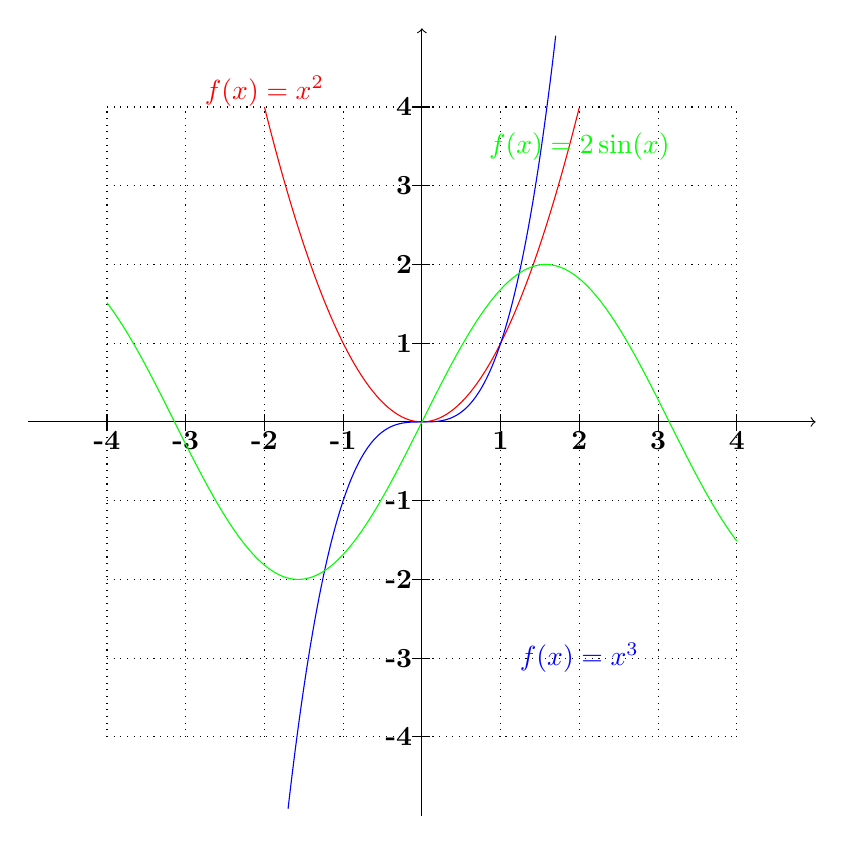
\begin{tikzpicture}
    
    \draw[->] (-5,0) -- (5,0);
    \draw[->] (0,-5) -- (0,5);
    
    \foreach \x in {-4,-3,-2,-1,1,2,3,4} {
        \draw [-] (\x,0.1) -- (\x,-0.1);
        \node[below] at (\x,0) {{\bf \x}};
        \draw [-] (-0.1,\x) -- (0.1,\x);
        \node[left] at (0,\x) {{\bf \x}};
    }
    
    \draw[dotted] (-4,-4) grid (4,4);
    
    % curves
    
    \draw[domain=-2:2,samples=300,color=red] plot ({\x},{\x*\x});
    \node at (-2, 4.2) {\textcolor{red}{$f(x)=x^2$}};
    
    \draw[domain=-1.7:1.7,samples=300,color=blue] plot ({\x},{\x*\x*\x});
    \node[color=blue] at (2,-3) {$f(x)=x^3$};
    
    \draw[domain=-4:4,samples=300,color=green] plot ({\x},{2*sin(\x r)});
    \node[color=green] at (2,3.5) {$f(x)=2\sin(x)$};
    
\end{tikzpicture}

\newpage

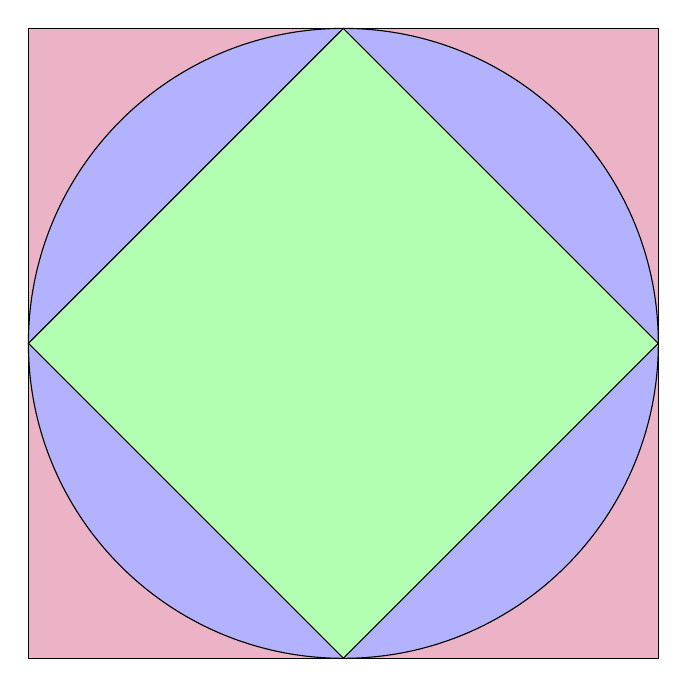
\begin{tikzpicture}
	
    \draw[fill=purple!30] (45:5.66) rectangle (225:5.66);
    \draw[fill=blue!30] (0:0) circle (4cm);
    \draw[fill=green!30] (90:4) -- (180:4) -- (270:4) -- (0:4) -- cycle;
   

\end{tikzpicture}

\newpage

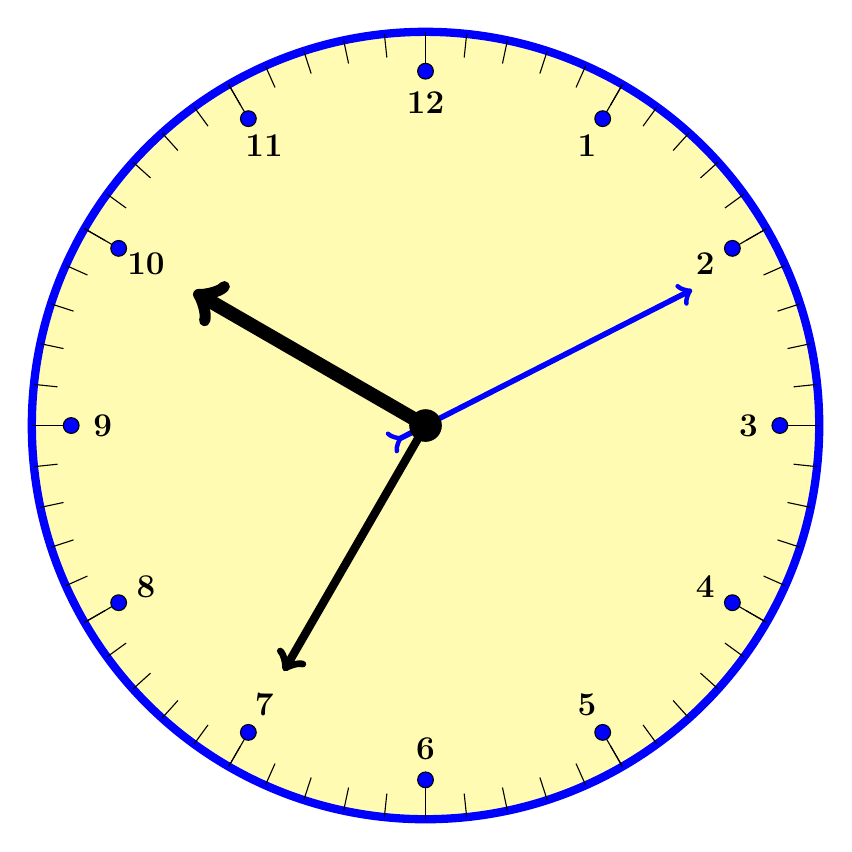
\begin{tikzpicture}

    \draw[color=blue,fill=yellow!30,line width=3pt] (0:0) circle (5cm);
    \foreach \x in {30,60,...,360} {
    	\draw ({\x}:4.6) -- ({\x}:5);
    	\draw[fill=blue] ({\x}:4.5) circle (1mm);
    	}
    \foreach \x in {0,6,...,360} {
    	\draw ({\x}:4.7) -- ({\x}:5);
    	}
    		
    \foreach \x in {1,2,...,12} {
    	\node at ({\x*-30+90}:4.1) {{\bf \large \x}};}
    
    
    \draw[->=stealth' , line width=5pt] (150:0) -- (150:3.4);
    \draw[->=stealth' , line width=3pt] (0:0) -- (240:3.6);
    \draw[>->=stealth' , line width=2pt, color=blue] (27:-0.5) -- (27:3.8);
    \draw[fill=black] (0:0) circle (0.2cm);

\end{tikzpicture}

\newpage

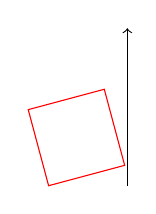
\begin{tikzpicture}
	\draw[color=red, rotate=15] (0,0) rectangle (1,1);
	\draw[->, xshift=1 cm] (0,0) -- (0,2);

\end{tikzpicture}

\newpage

\begin{animateinline}[controls]{1}
\multiframe{120}{rx=0+6} {

\begin{tikzpicture}

%    \draw[fill=purple!30] (45:5.66) rectangle (225:5.66);
%    \draw[fill=blue!30] (0:0) circle (4cm);
%    \draw[fill=green!30] (90:4) -- (180:4) -- (270:4) -- (0:4) -- cycle;


    \draw[color=blue,fill=yellow!30, line width=3pt] (0:0) circle (5cm);
    \foreach \x in {30,60,...,360} {
        \draw ({\x}:4.6) -- ({\x}:5);
        }
    \foreach \x in {0,6,...,360} {
        \draw ({\x}:4.6) -- ({\x}:5);
        }

    \foreach \x in {1,2,...,12} {
        \node at ({\x*-30+90}:4.2) {{\bf \large \x}};
        }




    \draw[->=stealth' ,rotate={90-\rx/3600}, line width=5pt] (0:0) -- (2.8,0); 
    \draw[->=stealth' ,rotate={90-\rx/60}, line width=3pt] (0:0) -- (3.8,0);
    \draw[>->=stealth' ,rotate={90-\rx}, line width=2pt, color=red] (0:0) --(4.2,0);


    \draw[fill=black] (0:0) circle (0.2cm);

\end{tikzpicture}}
\end{animateinline}

\newpage
\begin{animateinline}[controls]{100}
\multiframe{1200}{rx=0+1} {

\begin{tikzpicture}
    
    \draw[rotate={90-\rx}, line width=10pt] (-3,0) -- (0:0) -- (3,0);
    \draw[color=red, rotate=\rx, line width=10pt] (-3,0) -- (0:0) -- (3,0);
    \draw[color=blue, line width=7pt] (0:0) circle (3cm);
    
\end{tikzpicture}}
\end{animateinline}

\newpage


\begin{tikzpicture}


\end{tikzpicture}

\end{document}